% Preamble:
% \usepackage{tikz}
% \usepackage{subcaption}

\begin{figure}[ht]
\centering

% ---------------- (a) Simple graph ----------------
\begin{subfigure}[t]{0.47\textwidth}
\centering
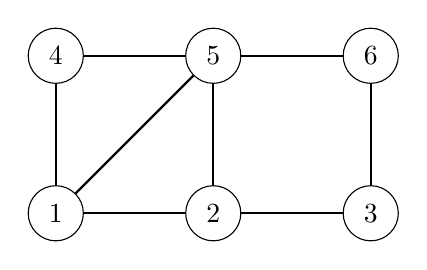
\begin{tikzpicture}[
  v/.style={circle, draw, minimum size=7mm},
  e/.style={thick}
]
% same 6 node positions for both subfigures
\node[v] (1) at (0,0) {1};
\node[v] (2) at (2,0) {2};
\node[v] (3) at (4,0) {3};
\node[v] (4) at (0,2) {4};
\node[v] (5) at (2,2) {5};
\node[v] (6) at (4,2) {6};

% simple graph edges (no loops, no parallel edges)
\draw[e] (1)--(2);
\draw[e] (2)--(3);
\draw[e] (1)--(4);
\draw[e] (2)--(5);
\draw[e] (3)--(6);
\draw[e] (4)--(5);
\draw[e] (5)--(6);
\draw[e] (1)--(5);

\end{tikzpicture}
\caption{Simple graph on 6 nodes}
\label{fig:simple6}
\end{subfigure}
\hfill
% ---------------- (b) Multigraph ----------------
\begin{subfigure}[t]{0.47\textwidth}
\centering
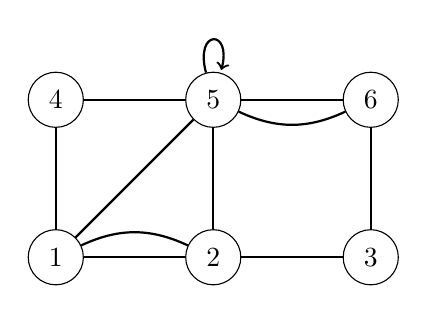
\begin{tikzpicture}[
  v/.style={circle, draw, minimum size=7mm},
  e/.style={thick}
]
% same 6 node positions
\node[v] (1) at (0,0) {1};
\node[v] (2) at (2,0) {2};
\node[v] (3) at (4,0) {3};
\node[v] (4) at (0,2) {4};
\node[v] (5) at (2,2) {5};
\node[v] (6) at (4,2) {6};

% base edges (same as simple graph, for comparison)
\draw[e] (1)--(2);
\draw[e] (2)--(3);
\draw[e] (1)--(4);
\draw[e] (2)--(5);
\draw[e] (3)--(6);
\draw[e] (4)--(5);
\draw[e] (5)--(6);
\draw[e] (1)--(5);

% parallel edges (multiedges)
\draw[e, bend left=25] (1) to (2);  % second edge between 1 and 2
\draw[e, bend right=25] (5) to (6); % second edge between 5 and 6

% a loop (allowed in many multigraph definitions)
\draw[e] (5) edge[loop above] (5);

\end{tikzpicture}
\caption{Multigraph on the same 6 nodes}
\label{fig:multi6}
\end{subfigure}

\caption{A simple graph versus a multigraph on the same vertex set. The multigraph includes parallel edges and a self-loop.}
\label{fig:simple-vs-multigraph}
\end{figure}
